\section{Problem Formulation} \label{sec:problem-formulation}

\begin{figure}[t!]
\centering
\begin{minipage}[t]{0.48\textwidth}
\centering
\vspace{0pt}
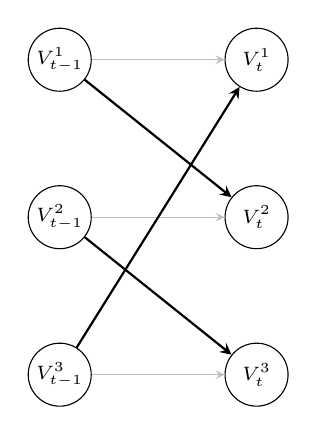
\begin{tikzpicture}[
    every node/.style={draw, circle, minimum size=0.8cm, font=\scriptsize, inner sep=0pt},
    >=stealth,
    ->,
    solidedge/.style={->, thick},
    temporal/.style={->, gray!50},
]

% t-1
\node (V1t1) at (0,4) {$V^1_{t-1}$};
\node (V2t1) at (0,2) {$V^2_{t-1}$};
\node (V3t1) at (0,0) {$V^3_{t-1}$};

% t
\node (V1t) at (2.5,4) {$V^1_t$};
\node (V2t) at (2.5,2) {$V^2_t$};
\node (V3t) at (2.5,0) {$V^3_t$};

% Temporal arrows (gray)
\foreach \i in {1,2,3} {
  \draw[temporal] (V\i t1) -- (V\i t);
}

% Causal edges (example)
\draw[solidedge] (V1t1) -- (V2t);
\draw[solidedge] (V2t1) -- (V3t);
\draw[solidedge] (V3t1) -- (V1t);

\end{tikzpicture}

\vspace{0.3em}
\textbf{(a) Lagged causal graph ($\ell_{\max}=1$)}
\end{minipage}%
\hfill
\begin{minipage}[t]{0.48\textwidth}
\centering
\vspace{0pt}
\renewcommand{\arraystretch}{1.2}
\setlength{\tabcolsep}{6pt}

\textbf{(b) Lagged adjacency tensor slice at lag \(1\)} \\[0.3em]
\(\mathbb{A}^{(0)}\)
\vspace{1.5em}

\begin{tabular}{c|ccc}
 & $V^1_{t-1}$ & $V^2_{t-1}$ & $V^3_{t-1}$ \\
\hline
$V^1_t$ & 0 & 0 & \textbf{1} \\
$V^2_t$ & \textbf{1} & 0 & 0 \\
$V^3_t$ & 0 & \textbf{1} & 0 \\
\end{tabular}

\vspace{1.5em}
%\scriptsize
\textbf{Interpretation:} \(\mathbb{A}^{(0)}_{ji}=1\) indicates a directed edge \(V^i_{t-1} \!\rightarrow\! V^j_t\).  For \(\ell_{\max}=1\), the slice index is \(0\).
\end{minipage}
\vspace{0.5em}
\caption{Illustrative example of a three-variable lagged causal graph with \(\ell_{\max}=1\) (left) and its corresponding lagged adjacency tensor (right) of shape \([3,3,1]\). The tensor entry \(\mathbb{A}_{j,i,\ell_{\max}-\ell}\) indicates whether a directed causal edge from \(V^i_{t-\ell}\) to \(V^j_t\) exists.}
\label{fig:lagged-tensor-example}
\end{figure}

Formally, we seek to construct a \textit{pre-trained neural architecture capable of learning causal graphs from time-series data}. Recall from Section \ref{sec:setting} that the objective of causal discovery is to infer the underlying causal graph \(\mathcal{G} \sim \mathcal{D}\) of a dataset \(\mathcal{D} \sim \mathcal{P}_{\mathcal{D}}\). Our task is to build a \textit{large causal model} (LCM), a foundation model capable of performing causal discovery directly from time-series data, outputting a temporal causal DAG from varying input lengths, domains, and underlying causal mechanisms. Let \(\mathbf{X} = \{ \mathbf{X}_t \}_{t=1}^{n} \in \mathbb{R}^{n \times k}, \quad \mathbf{X}_t = (X_t^1, \ldots, X_t^k) \in \mathbb{R}^k\) denote a multivariate time series with \(n\) timesteps and \(k\) variables. The goal of an LCM is to infer a time-lagged causal graph that captures the directed temporal dependencies among the variables. Specifically:

%\begin{definition}[Large Causal Model]
A \textit{large causal model (LCM)} is a parametric function \(f_\theta\) mapping a multivariate time series \(\mathbf{X}\) to a \textit{lagged causal adjacency tensor}

\begin{equation}
\mathbf{X} \xrightarrow{f_\theta} \hat{\mathbb{A}},
\end{equation}

where \(\hat{\mathbb{A}} \in [0,1]^{k \times k \times \ell_{\max}}\). Each entry \(\hat{\mathbb{A}}_{j,i,\ell_{\max}-\ell}\) represents the model's confidence in the directed causal relationship \(X^i_{t-\ell} \to X^j_t\). The maximum lag \(\ell_{\max}\) is a fixed hyperparameter bounding temporal dependencies, analogous to assumptions in classical methods such as PCMCI \citep{runge2018causal}. The notation \(\hat{\mathbb{A}}_{ji\ell}\) implies \(j\) is the row/effect and \(i\) is the column/cause. The same notation convention applies to the ground truth adjacency tensor \(\mathbb{A}\).
%\end{definition}

Unlike large language models or time-series forecasting foundation models that rely on self-supervision, causal discovery \textit{lacks natural self-supervised signals}. The ground-truth causal structure cannot be inferred from data alone, as it is fundamentally unidentifiable without external assumptions or supervision. Therefore, training follows a \textit{supervised learning scheme}, where pairs of ground truth lagged causal graphs and corresponding time-series samples are provided, generated from a known TSCM. This is illustrated in Figure \ref{fig:lagged-tensor-example}. 

As in neural networks (Figure \ref{fig:nn-train-infer}), two distinct phases are involved: (i) \textit{training}, where the model learns to map time-series data to causal graphs by provided with pairs of time-series data and their corresponding causal graphs in order to minimize its loss function; and (ii) \textit{inference (causal discovery)}, where the model (in constant time), once trained, directly outputs the predicted causal graph for unseen time-series data in the form of a lagged adjacency tensor \(\hat{\mathbb{A}}\), that best approximates the ground truth \(\mathbb{A}\). Figure \ref{fig:lcm-train-infer} conceptually illustrates the training and inference phase.

\begin{figure}[t!]
  \centering
   \makebox[\textwidth][c]{%
    \includegraphics[width=1.3\textwidth]{images/figures/causal-foundation-model.pdf}
  }
  \caption{Training step (left) and inference (causal discovery) step (right) of a large causal model \(f_\theta\), represented as a sequence of blocks. During training, the model learns to map input time-series \(\mathbf{X}\) to causal graphs by minimizing a supervised loss between the predicted graph \(\mathcal{G}_{\text{pred}}\) and ground-truth \(\mathcal{G}_{\text{gt}}\). During inference, the pre-trained model directly outputs \(\mathcal{G}_{\text{pred}}\) for unseen inputs.}
  \label{fig:lcm-train-infer}
\end{figure}

To make the problem well-posed under a supervised learning setting, we assume (i) sufficient overlap between training and test distributions \citep{ke2023learning, stein2024embracing, wu2024sample}, (ii) causal assumptions (described in Table \ref{tab:causal-assumptions}), and (iii) bounded temporal dependencies via fixed \(\ell_{\max}\). This formulation highlights the need for large and diverse training collections of temporal data and their corresponding causal graphs. In practice, \(\hat{\mathbb{A}}\) corresponds to a \textit{soft prediction tensor}: it assigns a confidence score to each potential lagged edge rather than a hard decision. To evaluate performance against the ground truth, these scores are binarized via a thresholding operator \(\hat{\mathcal{G}} = 1\{\hat{\mathbb{A}} \geq \tau\}\) (elaborated in Chapter \ref{chap:training}). Different values of \(\tau\) yield different precision-recall trade-offs, summarized using ROC/AUC and related metrics in Chapter \ref{chap:results}. Additionally, in order to handle samples and TSCMs of varying number of samples, variables and lags, a padding mechanism must be implemented as in conventional foundation models. A thorough discussion of the above is provided in Chapter \ref{chap:architecture}.